\documentclass[11pt]{article}
\usepackage[margin=1in]{geometry}
\usepackage{amsmath,amssymb}
\usepackage{graphicx}
\usepackage{booktabs}
\usepackage{natbib}
\usepackage{microtype}
\usepackage[hidelinks]{hyperref}
\usepackage{setspace}
\onehalfspacing

\title{Wellbeing and the Social Fabric in a Heterogeneous-Agent Economy:\\ Policy-Induced Decoupling and the Limits of Smooth Coordination}
\author{Alessandro Conway\thanks{Draft. Built on a heterogeneous-agent model first developed in the author's master's thesis (Sciences Po, 2020). All parameters are sourced or calibrated to stated data targets; every number and figure is reproduced by a single Julia script in the public repository.}}
\date{\today}

\begin{document}
\maketitle

\begin{abstract}
\noindent I embed social cohesion into a standard incomplete-markets economy in which households split time between market work and contributing to a social public good. The model is disciplined throughout: preference parameters take quasi-experimental consensus values, the effort margin is calibrated to French time-use data, and the model then matches wealth facts it was not aimed at. Two results follow. First, a budget-balanced make-work-pay subsidy raises aggregate consumption by five and a half percent while eroding the public good by nearly five percent, and the incidence is regressive twice over: the lower-income group loses on the material dimension, through the lump-sum financing, and on the social dimension at once, while the higher-income group converts the social loss into a material gain. A planner using a single-index objective adopts the policy and sees none of this. Second, a discipline result: the social-multiplier tipping mechanism that this class of models is often built to deliver cannot survive measured labour-supply elasticities. At the Frisch consensus of one half there is no multiplicity at any social-return strength, because the smooth intensive margin cannot bend the aggregate response enough to fold it; the multiplicity reported in an earlier version of this model required an elasticity eight times the evidence. Where multiplicity can honestly live is in discreteness and concentration: a discrete participation margin in the tradition of Brock and Durlauf restores genuinely distinct equilibria, and homophilous belonging sustains weak group-level multiplicity. The welfare claim is conditional and deliberately so: if wellbeing is multidimensional, as the SAGE framework and the WELLBY literature hold, standard policy evaluation misses both the social cost and who bears it.
\end{abstract}

\section{Introduction}

Across much of the rich world, measures of social and economic prosperity have come apart. \citet{snower2020} document a decoupling: indicators of social affiliation and individual empowerment diverged from real income per capita across developed countries over 2007 to 2017. The same period saw the politics of left-behind places, where \citet{rodrik2018} argues that globalisation drove a wedge between groups able to take advantage of open markets and the rest, eroding social cohesion. These are facts about wellbeing that a focus on consumption or output does not capture.

At the same time, a literature has matured around the claim that wellbeing is not the same object as the utility that economic agents maximise. \citet{benjamin2014,benjamin2023} show that subjective wellbeing measures do not correspond to decision utility, and argue that recovering overall wellbeing requires measuring and aggregating its separate components. \citet{layard2023} push the corresponding policy unit, the wellbeing-adjusted life year. If welfare is genuinely multidimensional, single-index welfare analysis is not merely incomplete; it can reach the wrong distributional conclusions, because it cannot see movements that offset within its single number.

This paper asks what changes when social cohesion is taken seriously as a structural feature of a heterogeneous-agent economy, and what that implies for policy evaluation. I take the workhorse incomplete-markets model \citep{bewley1986,aiyagari1994} and let households allocate time between market work and contributing to a social public good, following the SAGE framework of \citet{snower2020}. The contribution to society is the time not worked, an interpretation the time-use data supports directly: in the French time-use survey, paid work and unpaid domestic and associative work are of comparable magnitude \citep{roy2012}. The value an agent places on the public good can rise with its size, a social multiplier in the sense of \citet{glaeser2003}.

The discipline is the point. Risk aversion is set to the meta-analytic consensus on intertemporal substitution \citep{havranek2015}, the labour-supply elasticity to the quasi-experimental consensus \citep{chetty2011}, the discount factor and interest rate to standard annual values consistent with a stationary wealth distribution, and the effort-disutility scale is calibrated so that the baseline work share of committed time matches the French time-use figure of 0.53. Nothing else is tuned. The model then matches a hand-to-mouth share of one third \citep{kaplan2014} and a wealth Gini of 0.55 against a French target of roughly 0.68 \citep{conway2025atlas}, neither of which it was aimed at.

Two results follow. The first is normative. I introduce a recognisable policy, a budget-balanced make-work-pay subsidy to labour income, the kind of activation policy that real governments use. It raises the return to effort, so households work more and contribute less. Aggregate consumption rises by five and a half percent; the public good falls by nearly five percent. The incidence is the sharp part. The subsidy is financed by a lump-sum tax, so its net material effect is regressive: the lower-income group pays the same tax but draws a smaller subsidy, and its material gain falls outright, while the higher-income group gains materially. Both groups lose the social dimension. The lower-income group therefore loses on every dimension at once, and the aggregate consumption gain that a single-index planner sees is produced by the higher-income group's material improvement. A planner maximising consumption adopts the policy; a planner who evaluates welfare as multidimensional wellbeing sees a tradeoff and a distribution that the first planner's objective cannot represent.

The second result is a discipline result, and it is reported with the same prominence precisely because it is negative. The social-multiplier complementarity can in principle generate multiple equilibria, a low-cohesion and a high-cohesion society at identical fundamentals, and an earlier version of this model delivered exactly that. The multiplicity does not survive the evidence. At the consensus Frisch elasticity of one half there is no fold in the equilibrium map at any social-return strength, up to values fifteen times the old bistable window; the earlier result required an elasticity of four, eight times the quasi-experimental consensus, because only an implausibly elastic effort margin lets the social feedback bend the aggregate response enough to fold it. I take this to be a general lesson for the emerging wellbeing-macro literature: coordination-trap accounts of social cohesion cannot rest on smooth intensive margins. Where multiplicity can honestly live is in discreteness and concentration. A prototype in which participation in the social sphere is a discrete choice with a minimum meaningful time commitment, in the tradition of \citet{brock2001}, restores genuinely distinct equilibria, a zero-participation society coexisting with a participating one, and a homophilous belonging channel sustains weak multiplicity at the group level. Building the participation model out is the subject of the sequel.

The claim is conditional throughout, and that is its strength. I do not argue that wellbeing is multidimensional. I show that if it is, standard analysis misses a distributional tradeoff, and I give the mechanism. This sidesteps the philosophical dispute over whether utility is welfare and isolates a structural point that any reader can check.

The paper sits at an intersection that is individually active but jointly sparse. The SAGE framework is, in its authors' words, an illustrative representative-agent exercise; the wellbeing-as-objective literature is largely empirical and applied; heterogeneous-agent macroeconomics is a mature toolkit \citep{kaplan2018} but is rarely paired with a multidimensional wellbeing objective. Putting them together, with the parametrisation discipline that the pairing demands, is the contribution.

\section{Model}

\subsection{Environment}

Time is discrete and there is a unit mass of infinitely lived households. A household is described by assets $a \ge 0$ and an idiosyncratic productivity state $z \in \{z_l, z_h\}$ that follows a Markov chain with transition matrix $\Pi$, obtained by Rouwenhorst discretisation \citep{rouwenhorst1995} of a log AR(1) process and normalised so that $\mathbb{E}[z]=1$. Markets are incomplete: households self-insure by holding a riskless asset at exogenous gross rate $R$. The interest rate is taken as given, as in the original SAGE model; closing the model in general equilibrium is left to a sequel.

Each period a household chooses consumption $c$, next-period assets $a' \ge 0$, and labour effort $e \in [0,1]$. The time not worked is a contribution to a social public good, $q = 1-e$. Agency $\alpha_z \in [0,1]$ governs how much of effort becomes income.

\subsection{Preferences and the social dimension}

Utility is additively separable between a consumption-and-effort material-gain term and a social-cohesion term:\footnote{The separable form is deliberate and load-bearing. Greenwood-Hercowitz-Huffman preferences \citep{ghh1988}, which place the effort cost inside the consumption bundle, eliminate the wealth effect on labour supply. Here the wealth effect is the mechanism: households with more assets have a lower marginal utility of consumption and so work less and contribute more, which is what makes the contribution margin respond to wealth and income type. Separable preferences retain that channel.}
\begin{equation}
u(c,e;z) = \underbrace{\Gamma\left(\frac{c^{1-\gamma}}{1-\gamma} - \phi\,\frac{e^{1+\psi}}{1+\psi}\right)}_{\text{material gain } U^c} + \; S(e;z,Q).
\end{equation}
The social term is the object of interest. I consider three forms,
\begin{equation}
S(e;z,Q) =
\begin{cases}
\Lambda B_z\, Q, & \text{additive,} \\
\kappa\,\Lambda B_z\,(1-e), & \text{warm-glow,} \\
\kappa\,\Lambda B_z\,Q\,(1-e), & \text{social multiplier,}
\end{cases}
\end{equation}
where $Q$ is the aggregate public good, $B_z$ a taste for cohesion by type, $\Lambda$ the weight on cohesion, and $\kappa$ the strength of the behavioural social return. In the additive case the social term is separable and does not enter the choice of effort; this is the canonical baseline, the form in the original SAGE illustrative model, in which cohesion is a welfare overlay only. The warm-glow form is a private return to contributing, the act of contributing valued in itself, and it makes effort respond to social cohesion without any aggregate feedback. The multiplier form makes the marginal return to contributing rise with how much others contribute, a strategic complementarity in the sense of \citet{glaeser2003}. The product form is the simplest such complementarity and should be read as a modelling choice, not as following from the framework. One identification note is stated openly: in decision utility only the product $\kappa \Lambda B_z$ is identified; $\Lambda$ is pinned separately only on the wellbeing side, where $\Lambda B_z Q$ enters experienced wellbeing.

A fourth form generalises the multiplier to homophilous belonging. Let $\bar{q}_g$ denote the mean contribution of the household's own group $g$ and $h \in [0,1]$ a homophily weight. The belonging aggregate is
\begin{equation}
A_g = (1-h)\,Q + h\,\bar{q}_g,
\end{equation}
so that $h = 0$ is pure bridging, belonging drawn from the whole economy and identical to the multiplier above, and $h = 1$ is pure bonding, belonging drawn only from one's own group. This operationalises the bonding-bridging distinction of \citet{putnam2000} and the homophily evidence of \citet{mcpherson2001} at the cost of one parameter; the equilibrium fixed point becomes one aggregate per group.

\subsection{Budget and policy}

The flow budget applies agency to labour income and carries the policy instrument:
\begin{equation}
c + a' = R\,a + (1+\tau)\,\alpha_z\, e\, z\, Z - T, \qquad a' \ge 0,
\end{equation}
where $\tau$ is a proportional make-work-pay subsidy to labour income, $T$ a lump-sum tax that finances it, and $Z$ an aggregate productivity multiplier equal to one in the stationary economy. The government budget balances, $T = \tau\,\mathbb{E}[\alpha_z e z]$. Setting $\tau = T = 0$ recovers laissez-faire.

\subsection{The public good and equilibrium}

The public good is the average contribution across the stationary distribution $\lambda$,
\begin{equation}
Q = \mathbb{E}_\lambda[\,1-e\,] = \int (1-e(a,z))\, d\lambda(a,z).
\end{equation}
With value function $V$, the household solves
\begin{equation}
V(a,z) = \max_{a'\ge 0,\; e\in[0,1]} \; u(c,e;z) + \beta \sum_{z'}\Pi(z,z')\,V(a',z'),
\end{equation}
subject to the budget, taking the social aggregate as given. A stationary equilibrium is a set of policies, a distribution $\lambda$ invariant under the policies and $\Pi$, and a public good $Q = \mathbb{E}_\lambda[1-e]$, with the government budget balanced. In the multiplier case, define the map from a guessed public good to the realised one, $G(Q) = \mathbb{E}_{\lambda(Q)}[1-e]$. Equilibria are fixed points $Q = G(Q)$, and their number is the subject of Section \ref{sec:multiplicity}.

\section{Solution and calibration}

The model is solved with a stable, fast Julia routine. Effort is discretised and folded into the per-period reward, so the only dynamic-programming action is next assets, and the resulting discrete dynamic programme is solved by policy iteration. Effort is taken from this joint optimum rather than re-optimised separately, which matters: re-optimising effort against an interpolated value function collapses it once the social term is behavioural. Next assets are then refined continuously with effort fixed, and the stationary distribution is computed exactly: the lottery transition of \citet{young2010} is iterated, with a dense repeated-squaring fallback that is unconditionally stable when the wealth dynamics mix slowly. The fallback is not cosmetic; a stalled iteration biased the baseline public good by 1.7 percentage points before it was caught. In the multiplier case an outer loop iterates on the social aggregate to a fixed point; with the policy, an outer loop iterates on the lump-sum tax for budget balance. A full solve takes a fifth of a second on a laptop.

Calibration is summarised in Table \ref{tab:calib}. Every parameter is either a published consensus value, a value calibrated to a stated data target, or openly swept. Risk aversion is two, matching the selective-reporting-corrected mean elasticity of intertemporal substitution of one half \citep{havranek2015}. The inverse Frisch is two, the quasi-experimental intensive-margin consensus of \citet{chetty2011}. The discount factor and interest rate are standard annual values, $\beta R = 0.979$; the knife-edge pair used in the thesis version made the wealth distribution depend on the numerical grid boundary under consensus curvature and had to be replaced. The effort-disutility scale is calibrated so that the baseline mean work share equals 0.53, the paid share of committed time in the French time-use survey, where paid work averages 3h24 and unpaid domestic and associative work 3h01 per day \citep{roy2012}. Agency and the cohesion taste are differentiated by education group and follow the thesis, which built them from OECD Better Life Index indicators of labour-market security, health, skills, and the quality of social support. The income process sits within the annual ranges surveyed by \citet{heathcote2010}. The social-return strength $\kappa$ is swept and characterised, since no clean dataset disciplines it; this is stated rather than hidden.

Two untargeted moments then come out close to data: the share of households at the borrowing constraint is 0.33, in the hand-to-mouth range documented by \citet{kaplan2014}, and the wealth Gini is 0.55, against roughly 0.68 in French data \citep{conway2025atlas} and roughly 0.38 in standard calibrations of this model class. The income Gini is understated at these two income states; separating education from income risk and adding a transitory component raises it to 0.27 to 0.33 in prototype runs, at the known one-asset cost that the hand-to-mouth share falls, the frontier that motivates the two-asset extension of \citet{kaplan2014}.

\begin{table}[t]
\centering
\caption{Calibration. Lower and higher education types where two values appear.}
\label{tab:calib}
\begin{tabular}{llcl}
\toprule
parameter & symbol & value & basis \\
\midrule
risk aversion & $\gamma$ & 2.0 & EIS $= 0.5$, \citet{havranek2015} \\
inverse Frisch & $\psi$ & 2.0 & Frisch $= 0.5$, \citet{chetty2011} \\
effort disutility & $\phi$ & 14.0 & calibrated: work share $0.53$, \citet{roy2012} \\
discount factor & $\beta$ & 0.96 & standard annual, \citet{aiyagari1994} \\
gross interest rate & $R$ & 1.02 & long-run real rate, \citet{holston2017} \\
agency & $\alpha_l, \alpha_h$ & 0.765, 0.911 & OECD BLI empowerment, by education \\
cohesion taste & $B_l, B_h$ & 0.80, 0.94 & OECD BLI social support, by education \\
material weight & $\Gamma$ & 1.0 & normalisation \\
cohesion weight & $\Lambda$ & 0.876 & thesis; flagged for re-estimation \\
income persistence & $\rho$ & 0.90 & annual range, \citet{heathcote2010} \\
income dispersion & $\eta$ & 0.10 & annual range, \citet{heathcote2010} \\
social strength & $\kappa$ & swept & no clean target; stated openly \\
homophily & $h$ & swept & bonding-bridging weight \\
\bottomrule
\end{tabular}
\end{table}

\section{Policy-induced decoupling}

I introduce a budget-balanced make-work-pay subsidy of 20 percent to labour income under behavioural social cohesion (warm-glow, $\kappa = 1$). Table \ref{tab:policy} reports aggregates and Figure \ref{fig:dec} the incidence. The subsidy raises the return to effort, so households work more and contribute less. Aggregate consumption rises by 5.5 percent; the public good falls by 4.7 percent and social cohesion with it.

\begin{table}[t]
\centering
\caption{A budget-balanced make-work-pay subsidy under behavioural social cohesion.}
\label{tab:policy}
\begin{tabular}{lccc}
\toprule
 & baseline & with subsidy & change \\
\midrule
aggregate consumption & 0.438 & 0.462 & up 5.5\% \\
public good $Q$ & 0.491 & 0.468 & down 4.7\% \\
material gain $U^c$, lower-income group & $-3.540$ & $-3.579$ & down \\
material gain $U^c$, higher-income group & $-2.467$ & $-2.406$ & up \\
social cohesion $U^s$, lower-income group & 0.344 & 0.328 & down 4.7\% \\
social cohesion $U^s$, higher-income group & 0.404 & 0.385 & down 4.7\% \\
\bottomrule
\end{tabular}
\end{table}

\begin{figure}[t]
\centering
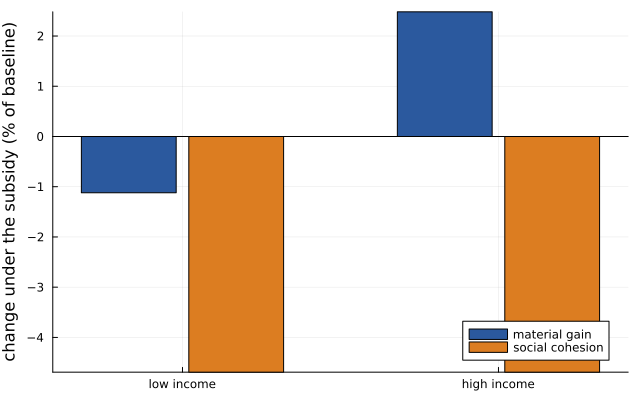
\includegraphics[width=0.62\textwidth]{figures/v11_decoupling_delta.png}
\caption{Incidence of the subsidy by group and dimension, in percent of the baseline level. The lower-income group loses on both dimensions; the higher-income group converts the social loss into a material gain.}
\label{fig:dec}
\end{figure}

The incidence is regressive twice over, and the financing is the reason. The lump-sum tax is the same for everyone while the subsidy is proportional to labour income, so the net material transfer is negative for the lower-income group: its material gain falls outright. The higher-income group's material gain rises, and since both groups bear the social erosion in proportion to their taste for cohesion, the lower-income group ends up worse on every dimension at once. The aggregate consumption gain that headline evaluation reports is produced by the higher-income group.

The contribution is the contrast between two planners ranking the same policy. A planner whose objective is aggregate consumption or decision utility sees the gain in the first row of Table \ref{tab:policy} and adopts the subsidy; neither the social cost nor its distribution appears in that objective. A planner who evaluates welfare as multidimensional wellbeing sees a tradeoff and sees who bears it. The claim is not that the policy is bad. It is that standard policy evaluation hides a distributional wellbeing cost that the structure of its objective cannot represent.

\section{Where multiple equilibria can and cannot live}
\label{sec:multiplicity}

A central promise of embedding social complementarities in macro models is multiplicity: a low-cohesion and a high-cohesion society at the same fundamentals, with history or expectations selecting. The multiplier form above can deliver this, and an earlier version of this model did. This section reports, with equal prominence, that the mechanism does not survive the evidence on labour supply, and locates where multiplicity can honestly live instead.

\subsection{The smooth intensive margin cannot fold}

Figure \ref{fig:nofold} shows the equilibrium public good against the social-return strength, solved from a low start and a high start, under two parametrisations. The left panel sets the Frisch elasticity to four, the value implicit in the thesis parametrisation. The branches split: a bistable window opens near $\kappa = 3.2$, with a low-cohesion equilibrium near 0.66 coexisting with a high-cohesion equilibrium near 0.98. The right panel sets the Frisch elasticity to the quasi-experimental consensus of one half \citep{chetty2011}. The branches coincide everywhere: a unique equilibrium at every strength tested, up to fifteen times the old window. The mechanics are transparent. The fold requires the aggregate contribution response to a change in the public good to be steep somewhere; the steepness is governed by the effort elasticity; at the measured elasticity the response is too flat to cross the diagonal more than once, at any feedback strength.

\begin{figure}[t]
\centering
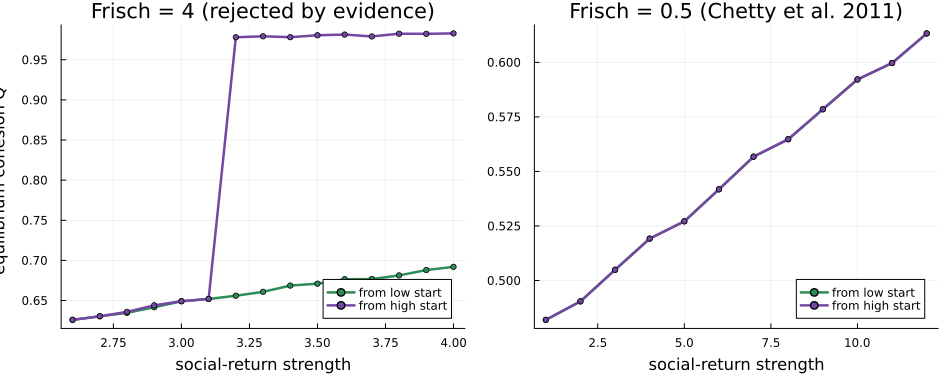
\includegraphics[width=0.95\textwidth]{figures/v11_nofold.png}
\caption{Equilibrium cohesion against social-return strength, from a low start (green) and a high start (purple). Left: at a Frisch elasticity of 4 the equilibrium map folds and a bistable window opens. Right: at the consensus elasticity of 0.5 the two branches coincide at every strength; there is no multiplicity to find.}
\label{fig:nofold}
\end{figure}

I report this as a result rather than burying it, for two reasons. First, the earlier version's multiplicity, and its corollary that tipping required agency inequality, were artefacts of an effort elasticity eight times the evidence; a referee would have found this, and the emerging wellbeing-macro literature should not build on it. Second, the diagnosis is constructive: it says precisely what a credible coordination account of social cohesion needs, namely a margin whose aggregate response can be steep without an implausible intensive-margin elasticity.

\subsection{Discreteness: the participation margin}

The theory of social interactions locates multiplicity in discrete choices with complementarities \citep{brock2001}. The natural discrete choice here is participation in the social sphere: one joins the association, the club, the commitment, with a minimum meaningful time lump, or one does not. This margin is also what the data measure: participation rates in associative life are around one third in France, and participants' social and volunteer time is of the order of a tenth of committed time. A prototype on the same engine makes participation a discrete choice with lump 0.10 and lets the belonging payoff rise with the participation rate. With a common threshold the economy is degenerate, all or nothing, exactly as the theory predicts for pure interaction payoffs. With a dispersed taste for belonging and a private warm-glow component anchoring the low equilibrium, since people volunteer even in low-participation places, the prototype already returns the quantitative question the sequel is built to answer: calibrating the interaction strength so that participation matches the French rate of one third, the economy sits inside the coordination region, with a low equilibrium near 15 percent participation coexisting with a high one near 50 percent when the private component is a third of the payoff, and the violence of the fold governed by that private share. At the low equilibrium only the highest-taste groups participate, the analogue of the education gradient in volunteering. Two caveats are stated plainly: near the fold the selected equilibrium is sensitive to the numerical grid, so the prototype establishes the structure of the region rather than point estimates, and the private share is not yet disciplined by data. Both are what the full build, with smoothed discrete choice and finer numerics, is for.

\subsection{Concentration: homophilous belonging}

The homophily channel gives a second, weaker source. Figure \ref{fig:hom} sweeps the homophily weight at a mid-range social strength. As belonging shifts from bridging to bonding, the groups' cohesion separates: the higher-education group's mean contribution rises and the lower-education group's falls, widening the gap by a third. The wellbeing incidence is regressive: moving from full bridging to full bonding raises the higher-education group's social wellbeing by nine percent and cuts the lower-education group's by nine percent, a structural rendering of the claim in \citet{putnam2000} that bridging social capital is what the disadvantaged lose most by its absence. At strong social strength and pure bonding, the lower-education group's own feedback loop sustains two stable cohesion levels two points apart depending on its own history, confirmed at tight tolerance: concentration of the feedback within a group partially restores, at the group level, what economy-wide smoothing destroys. The multiplicity is small; the distributional result is not.

\begin{figure}[t]
\centering
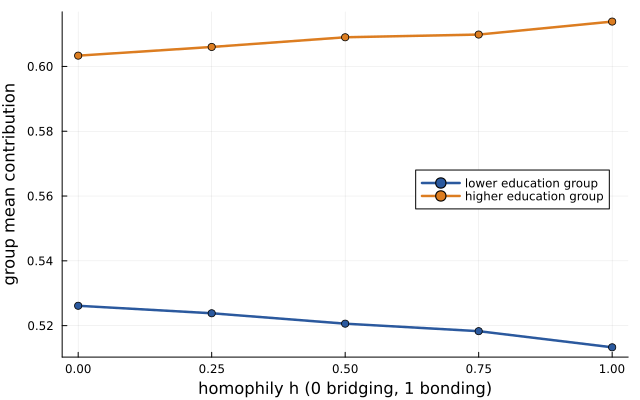
\includegraphics[width=0.62\textwidth]{figures/v11_homophily.png}
\caption{Group mean contribution against the homophily weight $h$ at $\kappa = 8$. Bonding-only belonging ($h = 1$) widens the cohesion gap between education groups; the lower-education group falls as the spillover from the more cohesive group is withdrawn.}
\label{fig:hom}
\end{figure}

\subsection{Composition: who carries the fabric}

Letting the population mix over social motives, in the proportions measured experimentally by \citet{fischbacher2001}, half conditional cooperators, a third free riders, a fifth unconditional givers, the economy settles at a cohesion level of 0.55, with the conditional cooperators carrying half the fabric and the givers over-contributing per head. Adding committed givers to a conditional population raises equilibrium cohesion with increasing returns, 0.07 percentage points per percentage point of givers at small shares, tripling at a thirty percent share, because givers seed the fabric that conditional cooperators then amplify. The composition results are levels, not switches; under measured elasticities a committed minority lifts the economy but cannot tip it.

\section{Welfare: decision utility versus experienced wellbeing}

The two-planner contrast rests on a distinction the recent literature has made precise. Decision utility is what households maximise. Experienced wellbeing is evaluated separately, over the dimensions material gain $U^c$ and social cohesion $U^s = \Lambda B_z Q$. \citet{benjamin2023} argue that subjective wellbeing is a function distinct from decision utility, and that recovering overall wellbeing requires aggregating its components. The two social objects in the model are deliberately not the same. What enters decision utility is the warm-glow or multiplier value of the act of contributing, the benefit that moves behaviour; what enters experienced wellbeing is $\Lambda B_z Q$, the enjoyment of the resulting public good. This is the framework's own distinction between contributing and receiving, and it is exactly the decision-utility versus experienced-wellbeing wedge that the empirical literature identifies.

I leave the wellbeing aggregator $W$ as an explicit modelling choice. The decoupling result is robust to that choice in a specific sense: any aggregator that treats the dimensions as imperfect substitutes, including the allostatic Leontief form $W = \min(U^c, U^s)$ up to scaling that the SAGE framework suggests, or a low-elasticity constant-elasticity form, registers a loss where the single-index objective registers a gain, and registers the lower-income group's double loss as the policy's first-order distributional fact. The non-substitutability is the substantive assumption and the main point of contestation, which is why the welfare claim is stated conditionally. The paper's logic is to take the multidimensional view seriously and trace its structural implications, not to adjudicate whether it is correct.

\section{Discussion and extensions}

Three extensions are designed and one is built. The built one is the homophily channel of Section \ref{sec:multiplicity}. The first designed extension is the participation model: discrete participation with taste dispersion and a private warm-glow anchor, calibrated to participation rates, which carries the coordination question on honest foundations and is the natural home of the agency dimension, since who can afford the participation lump is an agency question. The second is the general-equilibrium close, with a production side and transitions by the sequence-space Jacobian \citep{auclert2021}; that is also where the agency wedge, which here removes a fraction of labour income as a partial-equilibrium deadweight loss, should be given an explicit destination. The third folds a sustainability wedge into the material dimension, completing the framework's dimensions and aligning it with the wellbeing-accounting agenda \citep{hoekstra2019}. The model is built to take these on one at a time, sharing a single engine; in the prototypes above, every extension was either one engine parameter or an outer loop around the same solver.

The limitations are the partial-equilibrium structure, the swept social-return strength, the two-state income process of the headline calibration, and the modelling choice in the wellbeing aggregator. Each is stated rather than hidden, and the parametrisation discipline is the paper's answer to the obvious worry about a model with a social dimension: every number that can be tied to evidence is tied to it, and the two that cannot, $\kappa$ and $h$, are swept and characterised.

\section{Conclusion}

Embedding social cohesion in a disciplined heterogeneous-agent economy yields one robust policy result, one discipline result, and a programme. The policy result: a recognisable activation policy raises aggregate consumption while eroding the social fabric, and its incidence is regressive twice over, with the lower-income group losing on every dimension at once, a pattern that consumption-based evaluation structurally cannot see. The discipline result: the smooth social-multiplier route to multiple equilibria does not survive measured labour-supply elasticities, so coordination-trap accounts of social cohesion need discreteness, a participation margin, or concentration, homophilous belonging, both of which this paper prototypes. The programme: a modular engine in which agency, general equilibrium, and sustainability arrive one dimension at a time, calibrated against the wellbeing data that the empirical community already collects. If wellbeing is multidimensional, as the SAGE framework and the wellbeing literature hold, the structural model is the instrument that makes visible what single-index evaluation cannot represent, and the discipline applied here is what makes that instrument credible.

\bibliographystyle{plainnat}
\bibliography{references}

\end{document}
